%!TEX root = ../../main.tex
\subsection{Fraud Detection}
Fraud is a deliberate act of deception to access valuable resources~\cite{abdallah2016fraud}. The PwC global economic crime survey of 2018~\cite{Lavion2018,zhao2013fraud} found that half of the 7,200 companies they surveyed had experienced fraud of some nature. Fraud detection refers to detection of unlawfull activities across various industries, illustrated in Figure ~\ref{fig:AerasOfFraud}.

%%%%% Figure
\begin{figure}[h]
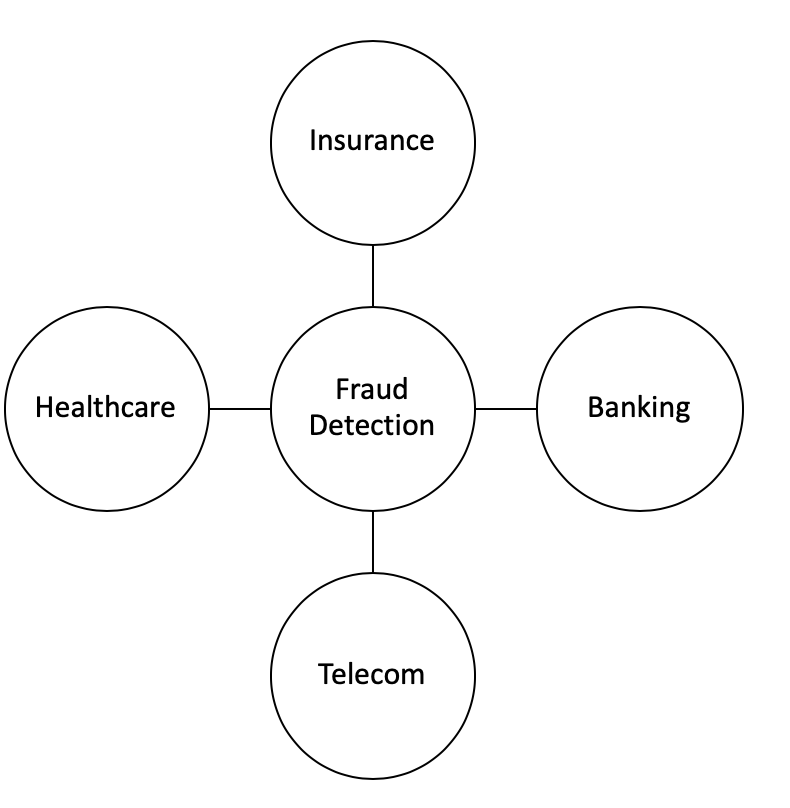
\includegraphics[scale=0.5]{images/AreasOfFraud}
\captionsetup{justification=centering}
\caption{Fraud detection across various application domains.}
\label{fig:AerasOfFraud}
\end{figure}
%%%%%%

Fraud in Telecom, insurance \textit{( health, automobile, etc)} claims, banking \textit{( tax return claims, credit card transactions etc)} represent significant problems in both governments and private businesses. Detecting and preventing fraud is not a simple task since fraud is an adaptive crime. Many traditional machine learning algorithms have been applied successfully in fraud detection~\cite{sorournejad2016survey}.  The challenge associated with detecting fraud is that it requires real time detection and prevention. This section focuses on deep anomaly detection (DAD) techniques for fraud detection.
%-----------------------------------------------------------------------------------------------------------

\subsubsection{Banking fraud:}
In the past decade, credit card was introduced in the banking sector. Now, credit card has become a popular
payment method in online shopping for goods and services. Credit card fraud involves theft of a payment card details, and use it as a fraudulent source of funds in a transaction. Many techniques for credit card fraud detection have been presented in the last few years~\cite{zhou2018state},~\cite{suganya2015survey}. Owing to the popularity of deep learning in various fields many techniques using deep learning models are proposed.
The challenge in credit card fraud detection is that frauds have no constant patterns. The typical approach in credit card fraud detection is to maintain a usage profile for each user and monitor the user profiles to detect any deviations. Since there are billions of credit card users this technique of user profile approach is not very scalabale. We will briefly review some of DAD techniques as shown Table~\ref{tab:creditfraudDetect}.
%%%%%%% Begin table fraud detection
\begin{table*}
\begin{center}
  \caption{Examples of Deep learning anomaly detection Techniques Used for credit card fraud detection.
          \\AE: Autoencoders, LSTM : Long Short Term Memory Networks
          \\RBM: Restricted Botlzmann Machines, DNN : Deep Neural Networks
          \\GRU: Gated Recurrent Unit, RNN: Recurrent Neural Networks
          \\CNN: Convolutional Neural Networks,VAE: Variational Autoencoders
          \\GAN: Generative Adversarial Networks}
  \label{tab:creditfraudDetect}
    \begin{tabular}{ | l | p{2cm} | p{7cm} |}
    \hline
    Technique Used & Section & References \\ \hline
     AE  & Section ~\ref{sec:ae}  & ~\cite{schreyer2017detection},~\cite{wedge2017solving} ,~\cite{paula2016deep},~\cite{renstrom2018fraud},~\cite{kazemi2017using},~\cite{zheng2018one},~\cite{pumsirirat2018credit} \\\hline
     RBM  & Section ~\ref{sec:dnn}  & ~\cite{pumsirirat2018credit} \\\hline
     DBN & Section ~\ref{sec:dnn} & ~\cite{seeja2014fraudminer} \\\hline
     VAE & Section ~\ref{sec:gan_adversarial} & ~\cite{sweers2018autoencoding} \\\hline
     GAN & Section ~\ref{sec:gan_adversarial} & ~\cite{fiore2017using},~\cite{choi2018generative} \\\hline
     DNN  & Section ~\ref{sec:dnn} & ~\cite{dorronsoro1997neural}, ~\cite{gomez2018end} \\\hline
     LSTM,RNN,GRU  & Section ~\ref{sec:rnn_lstm_gru} & ~\cite{wiese2009credit}, ~\cite{jurgovsky2018sequence} ,~\cite{heryadi2017learning},~\cite{ando2016detecting},~\cite{wang2017session},~\cite{alowais2012credit},~\cite{amarasinghe2018critical},~\cite{abroyan2017neural},~\cite{lp2018transaction}\\\hline
     CNN  & Section ~\ref{sec:cnn} & ~\cite{shen2007application},~\cite{chouiekh2018convnets},~\cite{abroyan2017convolutional},~\cite{fu2016credit},~\cite{lu2017deep},~\cite{wang2018credit},~\cite{abroyan2017neural} ,~\cite{zhang2018model}\\\hline
    \end{tabular}
\end{center}
\end{table*}
%%%%%%%%% End of table Banking detection




%-----------------------------------------------------------------------------------------------------------
\subsubsection{Mobile cellular network fraud:}
In recent times, mobile cellular networks  have witnessed  rapid deployment and evolution
supporting billions of users and a vast diverse array of mobile devices.
Due to this wide adoption and low mobile cellular service rates mobile
cellular networks is now faced with frauds such as voice scams targeted to steal customer private information, and messaging related scams to extort money from customers. Detecting such fraud is of paramount interest and not an easy task due to volume and velocity of mobile cellular network.
Traditional machine learning methods with static feature engineering  techniques fail to adapt to the nature of evolving fraud.
Table ~\ref{tab:mobilefraudDetect} lists DAD techniques for mobile cellular network fraud detection.

%%%%%%% Begin table fraud detection
\begin{table*}
\begin{center}
  \caption{Examples of Deep learning anomaly detection Techniques Used for mobile cellular network fraud detection.
          \\CNN:  convolution neural networks,DBN: Deep Belief Networks
          \\SAE: Stacked Autoencoders, DNN : Deep neural networks
          \\GAN: Generative Adversarial Networks }
  \label{tab:mobilefraudDetect}
    \begin{tabular}{ | l | p{2cm} | l | p{5cm} |}
    \hline
    Technique Used & Section & References \\ \hline
     CNN    & Section ~\ref{sec:cnn}  & ~\cite{chouiekh2018convnets} \\\hline
     SAE, DBN    & Section \ref{sec:ae}, Section ~\ref{sec:dnn}   &  ~\cite{alsheikh2016mobile},~\cite{badhe2017click} \\\hline
     DNN & Section ~\ref{sec:dnn}  &  ~\cite{akhter2012detecting},~\cite{jain2017perspective} \\\hline
     GAN & Section ~\ref{sec:gan_adversarial} &  ~\cite{zheng2018generative} \\\hline
    \end{tabular}
\end{center}
\end{table*}
%%%%%%%%% End of table fraud detection
%-----------------------------------------------------------------------------------------------------------
\subsubsection{Insurance fraud:}
Several traditional machine learning methods have been applied successfully to detect fraud in insurance claims ~\cite{joudaki2015using,roy2017detecting}. The traditional approach for fraud detection is based on features which are fraud indicators. The challenge with the traditional approaches is that the need of manual expertise. Another challenge is insurance fraud detection is the that the incidence of frauds is far less than the total number of claims, and also each fraud is unique in its own way. In order to overcome these limitations several deep anomaly detection techniques are proposed which are illustrated in Table ~\ref{tab:insurancefraudDetect}

%%%%%%% Begin table fraud detection
\begin{table*}
\begin{center}
  \caption{Examples of Deep learning anomaly detection Techniques Used for insurance fraud detection.
          \\DBN: Deep Belief Networks, DNN : Deep Neural Networks
          \\CNN: Convolutional Neural Networks,VAE: Variational Autoencoders
          \\GAN: Generative Adversarial Networks}
  \label{tab:insurancefraudDetect}
    \begin{tabular}{ | l | p{2cm} | l | p{5cm} |}
    \hline
     DBN & Section ~\ref{sec:dnn} & ~\cite{viaene2005auto} \\\hline
     VAE & Section ~\ref{sec:gan_adversarial} & ~\cite{fajardo2018vos} \\\hline
     GAN & Section ~\ref{sec:gan_adversarial} & ~\cite{fiore2017using},~\cite{choi2018generative} \\\hline
     DNN & Section ~\ref{sec:dnn} &~\cite{keung2009neural}\\\hline
     CNN  & Section ~\ref{sec:cnn} & ~\cite{shen2007application},~\cite{zhang2018model}\\\hline
    \end{tabular}
\end{center}
\end{table*}
%%%%%%%%% End of Insurance fraud
% \ref{sec:dnn}
% \ref{sec:stn}
% \ref{sec:spn}
% \ref{sec:word2vec}
% \ref{sec:gan_adversarial}
% \ref{sec:cnn}
% \ref{sec:rnn_lstm_gru}
% \ref{sec:ae}
%-----------------------------------------------------------------------------------------------------------
\subsubsection{Health insurance fraud:}

Healthcare is an integral component in people's lives, waste, abuse and fraud drive up costs in healthcare by tens of billions of dollars each year. Healthcare insurance claims fraud is a major contributor to increased healthcare costs, but its impact can be mitigated through fraud detection. Several machine learning models have been used effectively in health care insurance fraud~\cite{bauder2017medicare}.
This section presents the overview of deep learning based anomaly detection methods for healthcare fraud identification.
%%%%%%% Begin table fraud detection
\begin{table*}
\begin{center}
  \caption{Examples of Deep learning anomaly detection Techniques Used for health care fraud detection.
          \\RBM: Restricted Botlzmann Machines, GAN: Generative Adversarial Networks}
  \label{tab:healthcarefraudDetect}
    \begin{tabular}{ | l | p{2cm} | l | p{5cm} |}
    \hline
    Technique Used & Section & References \\ \hline
     RBM & Section ~\ref{sec:dnn} & ~\cite{lasaga2018deep} \\\hline
     GAN & Section ~\ref{sec:gan_adversarial} & ~\cite{ghasedi2018semi},~\cite{finlayson2018adversarial}\\\hline
     CNN  & Section ~\ref{sec:cnn} & ~\cite{esteva2017dermatologist}\\\hline
    \end{tabular}
\end{center}
\end{table*}
%%%%%%%%% End of table health care fraud

%-----------------------------------------------------------------------------------------------------------
